\chapter{Дифференцируемый рендеринг разреженных SDF}
\label{ch:chap2}

Базовый метод физически обоснованного дифференцируемого
рендеринга~\cite{Relax2024} предлагает простую оценку граничного интеграла для
функций расстояния со знаком (SDF) --- представления, более гибкого для
реконструкции поверхности, чем полигональный меш. Тем не менее ему присущ ряд
существенных ограничений. Во-первых, использование регулярной сетки приводит к
быстрому росту объёма модели: после каждой эпохи оптимизации размер сетки
увеличивается в 8~раз, что жёстко ограничивает допустимое число эпох при
ограниченном объёме памяти. Во-вторых, классический поиск пересечений методом
sphere tracing замедляет отрисовку. В-третьих, даже при локальном изменении
значений вблизи поверхности существующие реализации на каждом шаге оптимизации
запускают ресурсоёмкий алгоритм редистансинга, пересчитывая все значения
сетки, поскольку после обновления весов она перестаёт задавать корректную
функцию расстояния.

Для преодоления этих ограничений в работе предлагается метод дифференцируемого
рендеринга разреженных SDF-представлений. Опираясь на метод релаксированной
границы как на базовый, он перерабатывает ключевые этапы конвейера оптимизации
и вводит новые алгоритмы, адаптированные к разреженной структуре данных (см.
\hyperref[fig:comp]{Рисунок~\ref*{fig:comp}}). Метод опубликован в трудах
конференции IJCAI~2026 (уровень A*)~\cite{Budak2026SparseDR}. Его основной
вклад состоит в следующем:

\begin{figure}[ht]
    \centering
    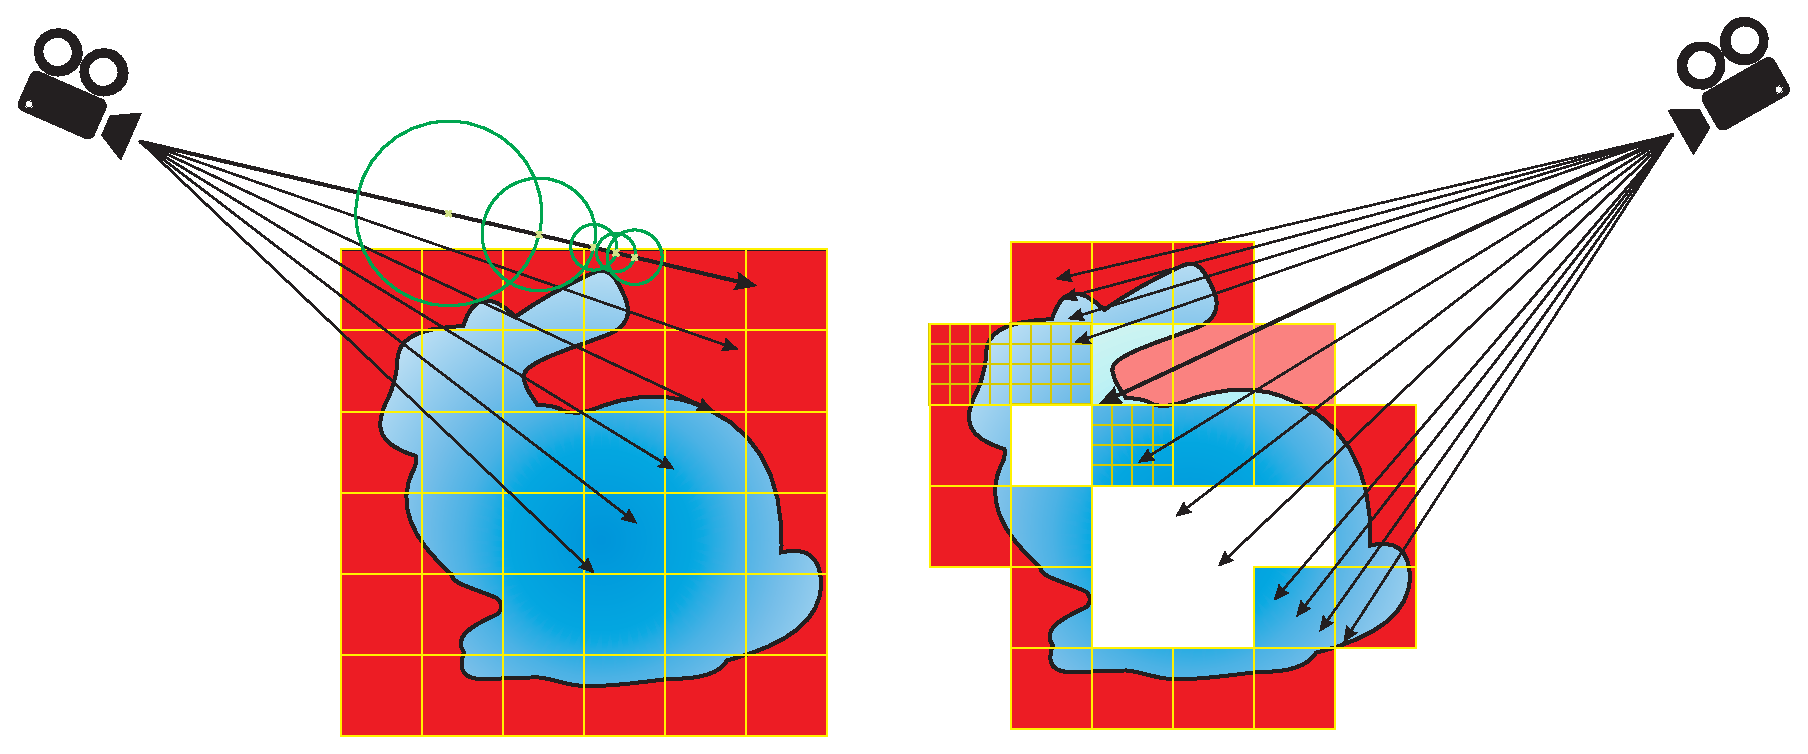
\includegraphics[width=\textwidth]{header.eps}
    \caption{Существующие методы (слева) используют регулярную SDF-сетку для представления поверхности, sphere tracing для пересечения лучей со сценой и равномерную выборку по изображению при проецировании лучей. Предложенный метод (справа) опирается на разреженное множество бриков (небольших SDF-сеток), при котором луч последовательно пересекает брики на своём пути до достижения поверхности, а также применяет адаптивную выборку для граничного интеграла, направляя больше лучей в область релаксированной границы. Красный и синий цвета соответствуют положительным и отрицательным значениям SDF}
    \label{fig:comp}
\end{figure}

\begin{enumerate}
    \item Адаптация дифференцируемого рендеринга SDF к разреженным
          представлениям, превосходящая базовый метод по скорости и замедляющая
          рост объёма модели: при каждом повышении разрешения размер
          разреженного представления увеличивается примерно в 4~раза против
          8~раз у плотной сетки, а на разрешении $2048^3$ оно оказывается в
          18--117~раз компактнее плотной сетки (см. главу~\ref{ch:chap4}).
    \item Две версии алгоритма редистансинга для разреженных представлений,
          одна из которых специально адаптирована под задачи дифференцируемого
          рендеринга.
\end{enumerate}

Процесс реконструкции организован в виде нескольких эпох, каждая из которых
включает несколько сотен итераций. На отдельной итерации сначала выполняется
отрисовка набора изображений с референсных ракурсов с одновременным накоплением
градиентов, затем к значениям дистанций применяется регуляризация, после чего
рассчитывается функция потерь относительно эталонных изображений, выполняется
обратное распространение ошибки и запускается локальный редистансинг. Между
эпохами SDF-сетка разреживается, её разрешение повышается, а затем выполняется
глобальный редистансинг.

В качестве представления геометрии используется разреженное множество бриков
(sparse brick set, SBS)~\cite{HanssonSoderlund} --- гибрид иерархической и
регулярной структур для функции расстояния со знаком. Оно строится как
BVH-дерево, в листьях которого хранятся брики (небольшие регулярные SDF-сетки).
Такая организация позволяет пропускать пустое пространство, отбрасывая листья,
не содержащие поверхности. При трассировке луч сначала обходит BVH-дерево, а при
попадании в лист пересекается с хранящейся в нём SDF-сеткой, последовательно
проходя листья на своём пути до пересечения с поверхностью либо до исчерпания
дерева. Помимо самой структуры SBS, в методе используются разработанные для неё
способы пересечения луча с вокселем --- метод Ньютона и аналитический метод,
адаптированные к поиску точек релаксированной границы для корректного расчёта
градиентов. Оба алгоритма используют тот факт, что внутри вокселя значение SDF
вдоль луча описывается кубическим полиномом, и различаются лишь способом
нахождения его корня. Поскольку точка релаксированной границы характеризуется
как локальный минимум SDF вдоль луча, её поиск внутри вокселя сводится к
нахождению нужного корня квадратного уравнения. При трилинейной интерполяции
локальный минимум нередко достигается на границе между вокселями, и этот случай
также явно обрабатывается.

Алгоритм реализован на языке C++ с использованием графического API Vulkan без
привлечения фреймворков автоматического дифференцирования --- все производные
выведены аналитически. Вычислительные шейдеры не пишутся вручную, а
генерируются из кода на C++ с помощью транслятора kernel\_slicer, причём
реализация поддерживает генерацию шейдеров на языке Slang. Чтобы обеспечить
произвольное число семплов на пиксель в шейдере оценки внутреннего интеграла,
производные распространяются блоками по 16~семплов. Для каждого семпла в стеке
фиксированного размера сохраняется информация о посещённых вокселях, а
производная функции потерь по цвету пикселя вычисляется по цвету, накопленному
к завершению блока: поскольку число семплов задаётся пользователем и заранее
неизвестно, хранить данные обо всех семплах пикселя одновременно в общем случае
невозможно. Если число семплов на пиксель не превышает размер блока, все они
обрабатываются совместно, и градиент вычисляется по итоговому цвету пикселя без
каких-либо приближений. Во всех проведённых экспериментах используется
16~семплов на пиксель (один блок), поэтому градиенты внутреннего интеграла
вычисляются точно. При большем числе семплов регулярная сетка внутри пикселя
обходится в порядке кривой Мортона, чтобы каждый блок равномерно покрывал весь
пиксель.

% Редистансинг

\begin{figure}[ht]
    \centering
    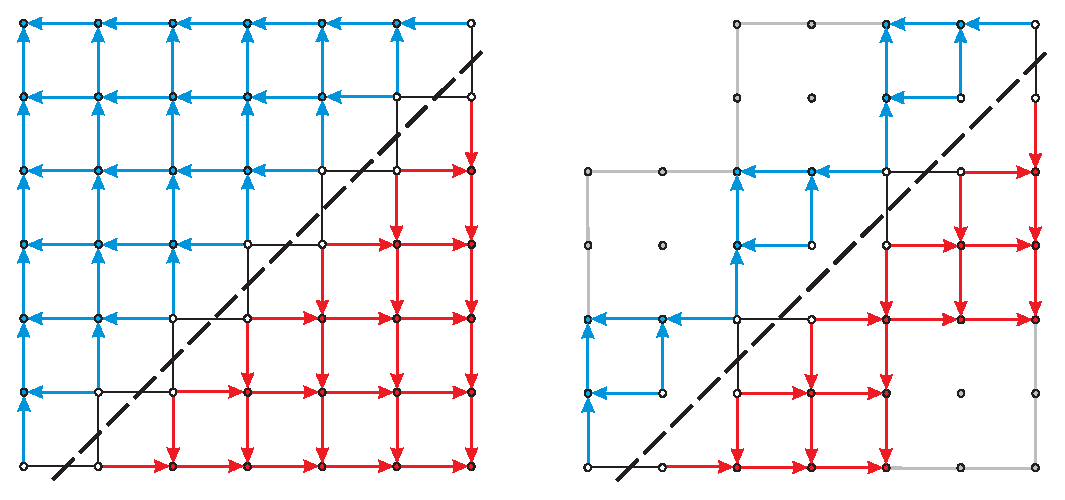
\includegraphics[width=0.9\textwidth]{redistancing.eps}
    \caption{Сравнение глобального алгоритма редистансинга на плотной сетке (слева) с локальным редистансингом для SBS (справа) при размере бриков $3\times 3$ дистанции. Точки обозначают значения дистанций: красные --- вне объекта, синие --- внутри объекта; пунктирная линия соответствует поверхности, заданной белыми точками. Стрелки указывают порядок обновления значений. Локальный редистансинг игнорирует брики без поверхности (выделены серым)}
    \label{fig:redist}
\end{figure}

После шага градиентного спуска обновлённые значения, строго говоря, перестают
задавать корректную SDF: они отклоняются от истинных расстояний до поверхности,
и сетка нарушает уравнение Эйконала. В базовом методе для восстановления этого
свойства применяется алгоритм редистансинга на основе метода fast
sweeping~\cite{RedistFSM}. Перенос данного этапа на разреженные представления
нетривиален: при пересчёте значений в одном брике необходимо находить и
учитывать соседние брики, даже если между ними нет непосредственного контакта
(промежуточные брики могли быть удалены как не содержащие поверхности, но
соседний брик по-прежнему влияет на корректные расстояния).

Полноценной адаптацией алгоритма под SBS служит глобальный редистансинг,
состоящий из трёх этапов. На первом этапе инициализируются значения вблизи
поверхности --- в узлах, у которых хотя бы один сосед вдоль координатной оси
имеет противоположный знак. По разностям с такими соседями оцениваются
допустимые границы расстояния до поверхности, и значение корректируется только
при выходе за эти пределы; остальные узлы инициализируются бесконечностью с
сохранением знака. На втором этапе выполняется метод fast sweeping: восемь
проходов с различными направлениями обхода, в каждом из которых брики
обрабатываются параллельно, а граничные значения соседних бриков считываются из
их состояния на начало прохода. Значения на общих гранях хранятся в одном
экземпляре и обновляются одним бриком-владельцем, благодаря чему результат не
зависит от порядка выполнения потоков. На третьем этапе для граней, не имеющих
примыкающего соседа и не содержащих поверхности, в расширяющейся окрестности
выполняется поиск ближайших бриков, после чего значения экстраполируются с
обращённых к ним граней соседей: выбирается минимум из текущего значения и суммы
расстояния между узлами с модулем значения в соседнем узле. Проходы fast
sweeping и экстраполяция повторяются до тех пор, пока остаются невычисленные
узлы. Распараллеливание выполняется по брикам, поскольку классические схемы
параллелизации fast sweeping опираются на порядок самих значений, что сложно
реализовать для SBS. Точность глобального и локального редистансинга в
сравнении с методом fast sweeping базового алгоритма приведена в
главе~\ref{ch:chap4} (Таблица~\ref{tab:redist}).

Важное преимущество аналитического метода и метода Ньютона при пересечении луча
с вокселем состоит в их меньшей чувствительности к точности дистанций по
сравнению со sphere tracing. Это позволяет отбрасывать воксель, если все его
значения превышают порог relaxed epsilon: в таком вокселе не может быть ни
пересечения с поверхностью, ни точки релаксированной границы. Следовательно,
точность дистанций в бриках без поверхности менее критична, и применять к ним
редистансинг на каждой итерации необязательно. На этом наблюдении основан
локальный редистансинг --- облегчённая версия алгоритма, выполняемая после
каждой итерации оптимизации (см. \hyperref[fig:redist]{Рисунок~\ref*{fig:redist}}).
Во-первых, пересчёт выполняется только в бриках, содержащих поверхность.
Во-вторых, предполагается, что значения внутри такого брика определяются лишь
фрагментом поверхности в нём самом: проходы fast sweeping ограничиваются
пределами одного брика без обращений к соседям, что упрощает алгоритм и
повышает локальность вычислений без потери качества реконструкции. Соседние
брики привлекаются только на этапе инициализации у поверхности: для узлов на
гранях используются соседи из примыкающего брика, а значение изменяется лишь
при выходе за границы, допустимые по соседям противоположного знака, что
предотвращает дрейф поверхности при многократном редистансинге. Поскольку общие
грани соседних бриков хранятся в единственном экземпляре, согласованность
дистанций на границах обеспечивается по построению, а результат не зависит от
порядка обработки бриков потоками.

При фиксированном разрешении SDF оптимизация выходит на плато за несколько
сотен итераций. Для дальнейшего повышения качества реконструкции необходимо
увеличивать разрешение сетки --- именно этот шаг разделяет эпохи оптимизации.
Итоговая детализация модели напрямую зависит от того, сколько эпох удаётся
выполнить при сохранении приемлемых затрат памяти и времени итерации. Для SBS
повышение разрешения заключается в разбиении каждого брика на восемь новых,
содержащих то же число дистанций, но покрывающих в восемь раз меньший объём.
Одновременно выполняется разреживание сетки: брики добавляются и удаляются так,
чтобы в представлении оставались только брики с поверхностью и окружающий их
буферный слой пустого пространства толщиной в один брик.

Примеры реконструкции предложенным методом для модели Dragon и скана бюста
Нефертити показаны на \hyperref[fig:exampl]{Рисунке~\ref*{fig:exampl}}.
Представлены результаты первой, третьей и седьмой (финальной) эпох вместе с
эталонным изображением.

\begin{figure}[ht]
    \centering
    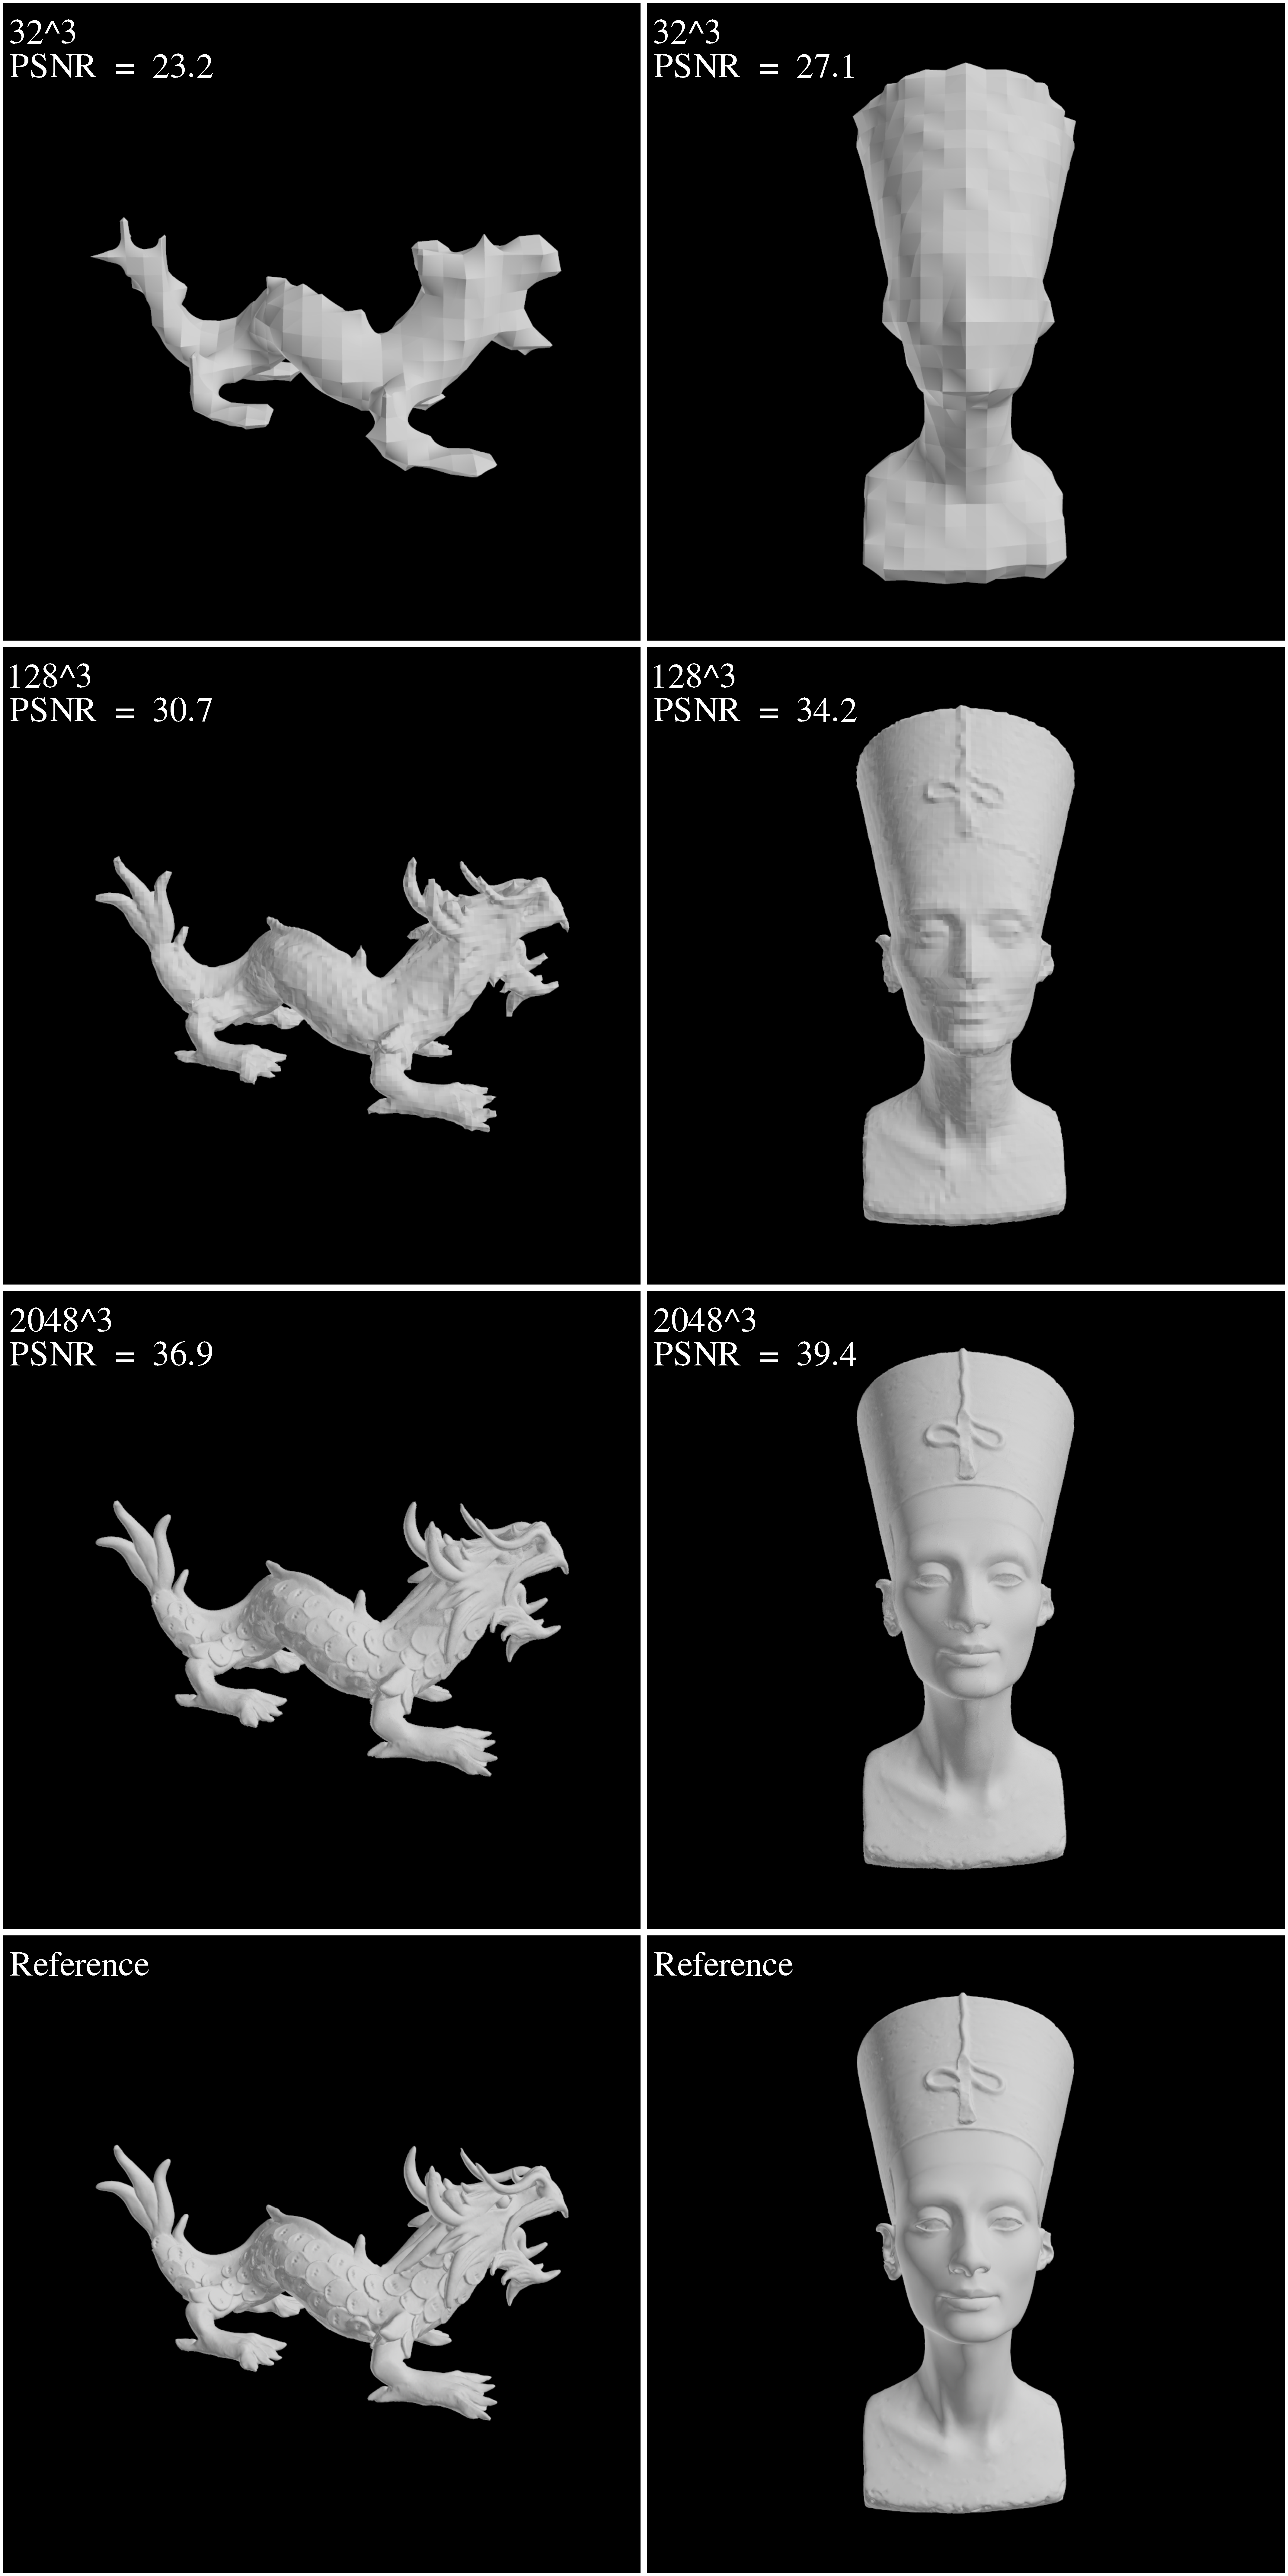
\includegraphics[width=0.75\textwidth]{collage_sparsedr.pdf}
    \caption{Примеры реконструкции для разных разрешений SBS}
    \label{fig:exampl}
\end{figure}


\endinput
